\documentclass[11pt,a4paper,twoside]{article}
\usepackage{a4wide}
\usepackage{amsmath}
\usepackage{amssymb}
\usepackage{amsthm}
\usepackage{graphicx}
\setlength{\parindent}{0pt}
\newcommand{\fracture}{\ensuremath{\gamma}}
\newcommand{\centerpoint}{\ensuremath{\boldsymbol{c}}}
\newcommand{\edge}{\ensuremath{e}}
\newcommand{\point}{\ensuremath{\boldsymbol{P}}}
\newcommand{\flux}{\ensuremath{u}}
\newcommand{\pressure}{\ensuremath{p}}
\newcommand{\edgepressure}{\ensuremath{\pi}}
\newcommand{\fracturetangent}{\ensuremath{\boldsymbol{t}}}
\newcommand{\fracturenormal}{\ensuremath{\boldsymbol{z}}}
\newcommand{\normal}{\ensuremath{\boldsymbol{n}}}
\newcommand{\normalarea}{\ensuremath{\boldsymbol{\nu}}}
\newcommand{\N}{\ensuremath{\rm N}}
\newcommand{\Narea}{\ensuremath{\tilde{\rm N}}}
\newcommand{\C}{\ensuremath{\rm C}}
\newcommand{\Smat}{\ensuremath{\rm S}}
\newcommand{\QC}{\ensuremath{\rm Q}_C^{\perp}}
\newcommand{\QCC}{\ensuremath{\rm Q}_C}
\newcommand{\QN}{\ensuremath{\rm Q}_N^{\perp}}
\newcommand{\PC}{\ensuremath{\rm P}_C^{\perp}}
\newcommand{\M}{\ensuremath{\rm M}}
\newcommand{\perm}{\ensuremath{\rm K}_I}
\newcommand{\trans}{\ensuremath{\rm T}}
\newcommand{\fluxvector}{\ensuremath{\boldsymbol{u}}}
\newcommand{\Mvel}{\ensuremath{{\rm M}_{\rm vel}}}
\newcommand{\cvect}{\ensuremath{\boldsymbol{g}}}
\newcommand{\centeredge}{\ensuremath{\boldsymbol{E}}}
\newcommand{\intsource}{\ensuremath{Q}}
\newtheorem{lemma}{Lemma}
\newtheorem{prop}{Proposition}

\author{Luca Formaggia}
\date{\today}
\title{A possible model for bifurcation in 2D fracture networks}
\begin{document}
\maketitle
\section{Geometrical construction}
We consider the case of three fractures $\gamma_i$, $i=0,1,2$, described as $2D$ curves that intersect. We make the following geometrical assumptions

\begin{enumerate}
\item The fractures intersect in a region that may be approximated by a triangle $I$;
\item In the vicinity of the intersection fractures may be assumed to
  be straight and with constant thickness. More precisely, there exist
  three points $\centerpoint_i$, with $i=0,1,2$, on each
  $\fracture_i$, respectively, such that the mid-line of fracture
  $\fracture_i$ (which we indicate with the same symbol) may be
  described in the vicinity of the intersection by equation
\begin{equation}
\label{eq:fracture}
\fracture_i=\fracture_i(s_i)=\centerpoint_i+s_i\fracturetangent_i \quad s_i\in (-S_1,S_i).
\end{equation}
Here, $\fracturetangent_i$ is the tangent vector to $\fracture_i$, $s_i$ is a
parameter and $S_i>0$ provides the bound so that the given expression
describes the fracture up to the intersection $I$.  In this portion of
the fracture the width $d_i$ is constant.  The situation is described
in figure \ref{fig:biforc1}.
\item \label{it:simple} A simplified setting is when we assume that
  the mid lines intersect at a single point $\centerpoint$. In that
  case we may take
  $\centerpoint_0=\centerpoint_1=\centerpoint_2=\centerpoint$. We will
  see that this stronger assumptions leads to some simplifications.
  See figure \ref{fig:biforc2}.
\item In the case of tee junction, we use the construction of figure
  \ref{fig:tee}. (WE NEED TO BE MORE PRECISE HERE).
\end{enumerate}

\subsection{Construction of the intersecting triangle}
We denote with $\fracturenormal_i$ the normal to $\fracture_i$ such
that the 2D cross product $\fracturetangent_i\times\fracturenormal_i$
is positive. We denote with $\fracture_i^{+}$ and $\fracture_i^{-}$
the borders of fracture $\fracture_i$ laying respectively opposite and
in the direction of $\fracturenormal_i$, as illustrated in the cited
figures.

We have that
\begin{equation}
\label{eq:fractureborders}
\fracture_i^{\pm}=\centerpoint_i + s_i\fracturetangent_i \pm \frac{d_i}{2}\fracturenormal_i,\quad i=0,1,2,\quad s_i\in (-S_1,S_i)
\end{equation}
We denote with $\point_{ji}$ the intersection of $\fracture_j^{-}$ and
$\fracture_i^{+}$, where $i=0,1,2$ and $j = (i+1)\mod 3$.
By simple calculations we have
\begin{equation}
\point_{ji}=\fracture_j^{-}(s_{ji}),
\end{equation}
where
\begin{equation}
\label{eq:pij}
s_{ji}=\left(
\left(
\centerpoint_i-\centerpoint_j+\dfrac{d_j}{2}\fracturenormal_j
\right)\cdot\fracturenormal_i+\dfrac{d_i}{2}
\right)/\fracturetangent_j\cdot\fracturenormal_i.
\end{equation}

If we adopt assumption \ref{it:simple} we have
\begin{equation}
\label{eq:pij}
s_{ji}=\left(
\dfrac{d_j}{2}\fracturenormal_j\cdot\fracturenormal_i+\dfrac{d_i}{2}
\right)/\fracturetangent_j\cdot\fracturenormal_i.
\end{equation}

\subsubsection{The case of the tee junction}
In the case of the tee junction, like that of figure \ref{fig:tee}
there are two indexes $i,j$, with $j=i+1 \mod 3$ such that
$\fracturetangent_j\cdot\fracturenormal_i=0$\footnote{In practice we
  identify the tee junction if
  $|\fracturetangent_j\cdot\fracturenormal_i|\le \tau$, $\tau$ being a
  suitable tolerance.}.

In this case we set
\begin{equation}
\label{eq:teepoint}
\point_{ji}=\frac{\centerpoint_j-(d_j/2)\fracturenormal_j +
\centerpoint_i+(d_i/2)\fracturenormal_i }{2}
\end{equation}

\subsection{Interface conditions}
To identify the interface conditions we consider the intersection
triangle $I$ we employ a mimetic hybridized finite difference scheme
\cite{lie2012open,brezzi2005family}.  We assume that triangle $I$ is
non degenerate and we refer to figure \ref{fig:triangle} for
notation. In particular we indicate with $\normal_i$ the outward
normal to $i-th$ triangle edge $\edge_i$, and we set\footnote{Note that the
  triangle nodes are numbered clockwise.}
\begin{equation}
\label{eq:normalarea}
\normalarea_i=|\edge_i|\normal_i,
\end{equation}
as the area (length) scaled normal. We indicate with $\centeredge_i$ the mid point of edge $\edge_i$ and we set
\begin{equation}
\label{eq:cvect}
\cvect_i=\centeredge_i-\centerpoint_I,
\end{equation} 
where here $\centerpoint_I$ is the center of mass of triangle $I$.  We
use notation inspired from \cite{lie2012open} since it is of immediate
implementation. In particular with $\flux_i$ we indicate the mass flux
across edge $\edge_i$. We not that a positive $\flux_i$ denotes a flux
that is exiting the triangle across the corresponding edge. We use the
mass flux as variable and not the average velocity as done elsewhere
because it is the quantity more readily interfaced with the reduced
model for the fracture network presented in \cite{Formaggia2014}. Of
course the expressions that follow can be recast using average
velocity by a simple rescaling.

\subsubsection{Preliminaries}
We introduce the following matrices
\begin{equation}
\label{eq:normalarea}
\N=\begin{bmatrix}
\normalarea_0^T\\\normalarea_1^T\\\normalarea_2^T
\end{bmatrix}
\quad \text{and }
\C=\begin{bmatrix}
\cvect_0^T\\\cvect_1^T\\\cvect_2^T,
\end{bmatrix}
\end{equation}
which are of dimension $3\times 2$.
\begin{prop}
The nullspace of both $\C^T$ and $\N^T$ is spanned by the constant vector
$\boldsymbol{1}_3=[1,1,1]^T$.
\end{prop}
\begin{proof}
The fact that 
\[
\N^T\boldsymbol{1}_3=\sum_{i=0}^3\normalarea_i=\boldsymbol{0}
\]
 and 
\[
\C^T\boldsymbol{1}_3=\sum_{i=0}^3\cvect_i=\boldsymbol{0}
\] 
is an immediate consequence of the fact that a triangle is a polygon and of the definition of the matrices.
 We need to prove that $\boldsymbol{1}_3$ generates the whole nullspace.
 The proof is analogous for the two matrices, so we consider just $\N$.

 Let assume that there is a non null vector $\boldsymbol{\alpha}=[\alpha_0,\alpha_1,\alpha_2]^T\ne \beta\boldsymbol{1}_3$
for any $\beta\in\mathbb{R}$ such that
\[
\N^T\boldsymbol{\alpha}_3=\sum_{i=0}^3\alpha_i\normalarea_i=\boldsymbol{0}.
\]
Without loss of generality we assume $\alpha_0\ne 0$. It means
that there exists two real numbers $a_1=\alpha_1/\alpha_0$ and $a_2=\alpha_2/\alpha_0$ such that
\[
\normalarea_0=-a_1 \normalarea_1 - a_2 \normalarea_2.
\]
Yet, we have already demonstrated that
\[
\normalarea_0=-\normalarea_1 -\normalarea_2.
\]
Then, $ (1-a_1)\normalarea_1=-(1-a_2)\normalarea_2$. Since all
$\normalarea_i$ are different from zero and
$\normalarea_1\ne\normalarea_2$ otherwise the triangle is degenerate,
we may conclude that the previous expression implies $a_1=a_2=1$, and
thus $\alpha_0=\alpha_1=\alpha_2$, which is excluded by hypothesis.
\end{proof}

As a consequence, $\QC=\QN=\frac{1}{\sqrt{3}}\boldsymbol{1}$ is the
$3\times 1$ matrix whose column is an orthogonal basis of
$\operatorname{ker}(\C^T)$ and $\operatorname{ker}(\N^T)$, respectively.

Let now $\QCC$ be the matrix whose columns form an orthogonal basis of
the image of $\C$. Since
$\operatorname{dim}(\operatorname{range}(\C))=3-
\operatorname{dim}(\operatorname{ker}(\C^T))=2$ the matrix is $3\times 2$.


\begin{prop}
The $3\times 3$ matrix 
\begin{equation}
\PC={\rm Id}_3 -\QCC\QCC^T
\end{equation}
represents the orthogonal projector on the null space of $\C^T$. As a consequence, for all $\boldsymbol{v}=[v_0,v_1,v_2]^T$
\begin{equation}
\label{eq:project}
\PC\boldsymbol{v}=\overline{v}\boldsymbol{1}_3,\quad \text{with }
\overline{v}=\dfrac{1}{3}\sum_{i=1}^{3}v_i.
\end{equation}
Here, ${\rm Id}_3$ is the $3\times 3$ identity matrix.
\end{prop}
\begin{proof}
  Indeed, the nullspace of $\QCC^T$ coincides with that of $\C^T$ by
  construction. Thus if $\boldsymbol{w}=\alpha\boldsymbol{1}_3$ for an
  arbitrary $\alpha\in\mathbb{R}$ we have, for any
  $\boldsymbol{v}\in\mathbb{R}^3$
\[
\boldsymbol{v}^T\PC\boldsymbol{w}=\boldsymbol{v}^T\boldsymbol{w}.
\]
which proves that $\PC$ is an orthogonal projector.

Since $\PC$ is an orthogonal projection on a space whose orthogonal basis
is formed just by the vector $\boldsymbol{k}=3^{-1/2}\boldsymbol{1}_3$ we have that
\begin{equation}
\label{eq:pc1}
\PC\boldsymbol{v}=(\boldsymbol{v}\cdot\boldsymbol{k})\boldsymbol{k}
=\overline{v}\boldsymbol{1}_3
\end{equation}
\end{proof}
\begin{prop}
Let ${\rm S}$ be a $3\times 3$ symmetric positive definite matrix, with elements $S_{sl}$. We have
\begin{equation}
\label{eq:pc2}
\PC {\rm S}\PC\boldsymbol{v}=\hat{s}\QC(\QC)^T\boldsymbol{v}=
\hat{s}\overline{v}\boldsymbol{1}_3,
\end{equation}
with 
\begin{equation}
\label{eq:shat}
\hat{s}=\dfrac{1}{3}\sum_{ls=0}^3S_{ls}
\end{equation}
\end{prop}
\begin{proof}
It is a simple application of the previous result and of the definition of $\QC$. 
\end{proof}
Therefore,
\[
\operatorname{rank}(\PC{\rm S}\PC)=1.
\]

\begin{figure}
\begin{center}
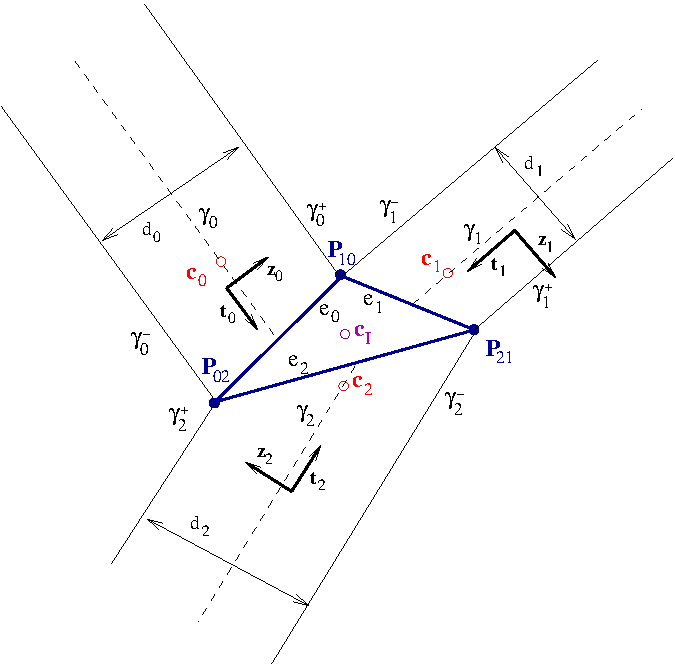
\includegraphics[width=0.6\textwidth]{Figure/biforc1}
\caption{\label{fig:biforc1}}
\end{center}
\end{figure}
\begin{figure}
\begin{center}
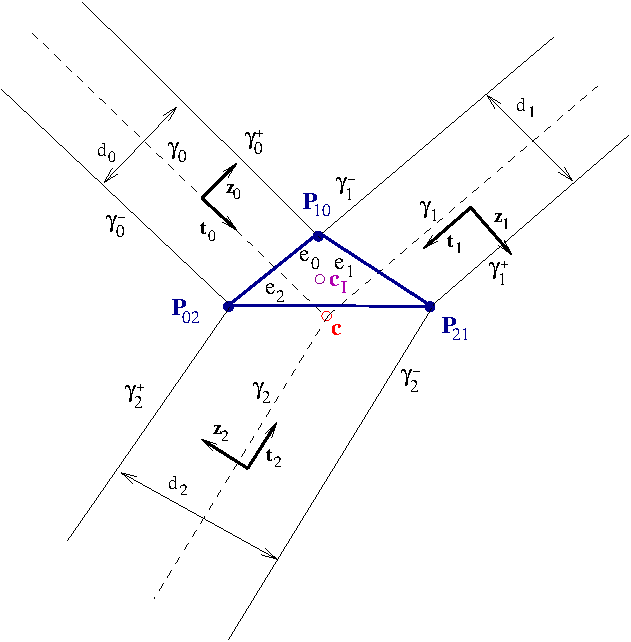
\includegraphics[width=0.6\textwidth]{Figure/biforc2}
\caption{\label{fig:biforc2}}
\end{center}
\end{figure}
\begin{figure}
\begin{center}
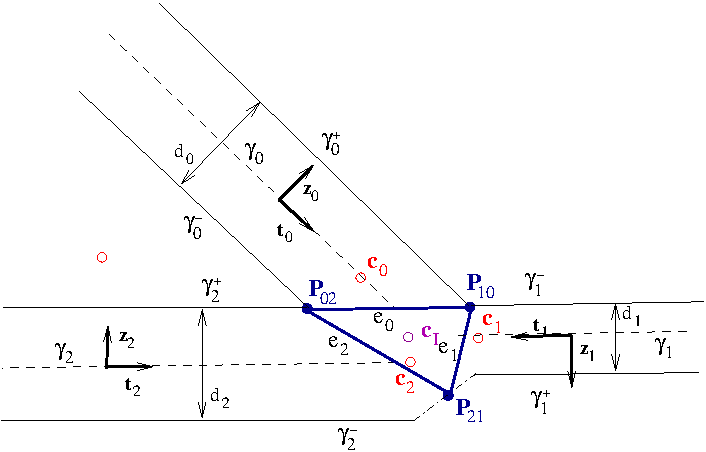
\includegraphics[width=0.6\textwidth]{Figure/tee}
\caption{\label{fig:tee}}
\end{center}
\end{figure}
\begin{figure}
\begin{center}
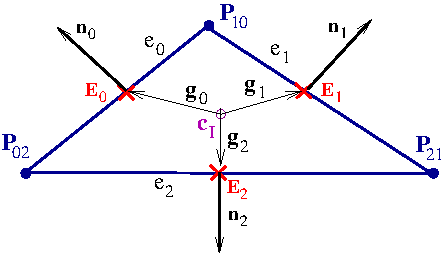
\includegraphics[width=0.6\textwidth]{Figure/triangle}
\caption{\label{fig:triangle}}
\end{center}
\end{figure}

\subsubsection{The derivation of the interface conditions}
Let $\perm$ be the symmetric $2\times 2$ matrix representing the
permeability at the intersection, $\pressure_I$ the pressure at the
intersection, located at $\centerpoint_i$ and $\edgepressure_i$,
$i\in\{0,1,2\}$ the Lagrange multipliers that represent the values of pressure
at $\centeredge_i$.

Let $\fluxvector=[\flux_0,\flux_1,\flux_2]^T$ be the vector of fluxes,
and $\Pi=[\edgepressure_0,\edgepressure_1,\edgepressure_2]^T$ that of
the edge pressures.  The application of a mimetic finite difference
scheme on the triangle $I$ for the Darcy's constitutive relation,
ignoring gravity effects, leads to a relation of the type
\begin{equation}
\label{eq:constitutive}
\fluxvector=\trans(\pressure_I\boldsymbol{1}_3-\Pi),
\end{equation}
where $\trans$ is the \emph{transmissibility matrix} that takes the general form
\begin{equation}
\label{eq:trans}
\trans=\dfrac{1}{|I|}\N\perm\N^T + \PC{\rm S}\PC,
\end{equation}
or, equivalently,
\begin{equation}
\label{eq:trans2}
\trans=\frac{1}{|I|}\N\perm\N^T + s\QC(\QC)^T=\dfrac{1}{|I|}\N\perm\N^T + \dfrac{s}{3}\mathcal{I},
\end{equation}
where $\mathcal{I}=\boldsymbol{1}_3\boldsymbol{1}_3^T$ is the matrix with all elements equal to $1$.
Here, ${\rm S}$ is a suitable symmetric positive definite matrix, and $s>0$ 
a constant.

Typical solutions are 
\begin{equation}
\label{eq:esse}
{\rm S}=t\operatorname{diag}(\N\perm\N^T)
\end{equation}
being $t>0$ a parameter (a possible value is $t=6$), or
\begin{equation}
\label{eq:esse}
{\rm S}=t\operatorname{trace}(\perm){\rm Id}_3
\end{equation}

\begin{prop}
Matrix $\trans$ is symmetric positive definite.
\end{prop}
\begin{proof}
  Indeed, by using (\ref{eq:pc1}), (\ref{eq:pc2}), and exploiting the
  symmetry of $\PC$, for any $\boldsymbol{v}\ne\boldsymbol{0}$
\[
\boldsymbol{v}^T\trans\boldsymbol{v}=
\dfrac{1}{|I|}\boldsymbol{v}^T\N\perm\N^T\boldsymbol{v}+
3\overline{v}^2\hat{s}.
\]
Now, $\hat{s}>0$ since ${\rm S}$ is s.p.d. and $\boldsymbol{v}^T\N\perm\N^T\boldsymbol{v}\ge 0$ since 
$\perm$ is s.p.d.. This concludes the proof.
\end{proof}

We now use the continuity equation $\nabla\cdot u=q$ in $I$, which in the mimetic difference framework is approximated as
\begin{equation}
\label{eq:continuity}
\sum_{i=0}^2 \flux_i=\boldsymbol{1}_3^T\fluxvector=\intsource, \quad \text{with } \intsource=\int_Iq\, d\Omega
\end{equation}
Using (\ref{eq:constitutive}) we have
\begin{equation}
\label{eq:continuity2}
\intsource=\boldsymbol{1}_3^T\fluxvector=\boldsymbol{1}_3^T\trans(\pressure_I\boldsymbol{1}_3-\Pi),
\end{equation}
We now use (\ref{eq:trans}) and (\ref{eq:pc2}) to obtain the following
\begin{prop}
We have that 
\begin{equation}
\label{eq:pressure}
\pressure_I=\dfrac{\intsource}{3\hat{s}}+\overline{\edgepressure},
\end{equation}
where $\overline{\edgepressure}=\frac{1}{3}\sum_{i=0}^2\edgepressure_i$.
In particular, in the absence of source terms $\pressure_I=\overline{\edgepressure}$.
\end{prop}
\begin{proof}
We start by noting, thank to symmetry, that
\[
\boldsymbol{1}_3^T\PC=\boldsymbol{1}_3^T\quad \text{and } \PC\boldsymbol{1}_3=\boldsymbol{1}_3.
\]
and we recall that
\[
\N\boldsymbol{1}_3=\boldsymbol{0}.
\]
Thus, by using (\ref{eq:pc2}) and the fact that $\overline{\boldsymbol{1}_3}=1$, we get
\[
\pressure_I\boldsymbol{1}_3^{T}\trans\boldsymbol{1}_3=\pressure_I\hat{s}\boldsymbol{1}_3^{T}\boldsymbol{1}_3=3\pressure_I\hat{s}.
\]
While,
\[
\boldsymbol{1}_3^{T}\trans\Pi=\boldsymbol{1}_3^{T}\trans\Pi=
\hat{s}\overline{\edgepressure}\boldsymbol{1}_3^{T}\boldsymbol{1}_3=3\hat{s}\overline{\edgepressure}.
\]
Substituting into (\ref{eq:continuity2}) we have
\[
3\hat{s}(\pressure_I-\overline{\edgepressure})=\intsource,
\]
which allows us to conclude the proof.
\end{proof}
Consequently, we have the following system
\begin{equation}
\label{eq:finalsystem}
\begin{cases}
\fluxvector-\pressure_I\trans\boldsymbol{1}_3-\trans\Pi=\boldsymbol{0}\\
\sum_{i=0}^2 \flux_i=\intsource \\
\pressure_I-\overline{\edgepressure}=\dfrac{\intsource}{3\hat{s}}.
\end{cases}
\end{equation}

When coupling with the reduced model of fractures we will identify 
$\flux_i$ and $\edgepressure_i$ as the fluxes (BEWARE OF THE SIGN CONVENTION)
and pressures at the end of the fracture located at the bifurcation. While,
$\pressure_I$ is the pressure at the bifurcation, which can be computed (if needed) as post-processing stage since system (\ref{eq:finalsystem}) is obviously equivalent to
\begin{equation}
\label{eq:finalsystem2}
\begin{cases}
\fluxvector-\trans\left(\overline{\edgepressure} \boldsymbol{1}_3-\Pi\right)=\dfrac{\intsource}{3\hat{s}}\trans\boldsymbol{1}_3\\
\sum_{i=0}^2 \flux_i=\intsource.
\end{cases}
\end{equation}

We finally recall that $\trans\boldsymbol{1}_3=\hat{s}\boldsymbol{1}_3$.

\bibliographystyle{plain}
\bibliography{bifurcation.bib}

\end{document}
%%% Local Variables: 
%%% mode: latex
%%% TeX-master: t
%%% End: 
